\newpage
\subsection{Caso d'uso UC3: Login da \progetto}
\label{UC3}
\begin{figure}[ht]
	\centering
	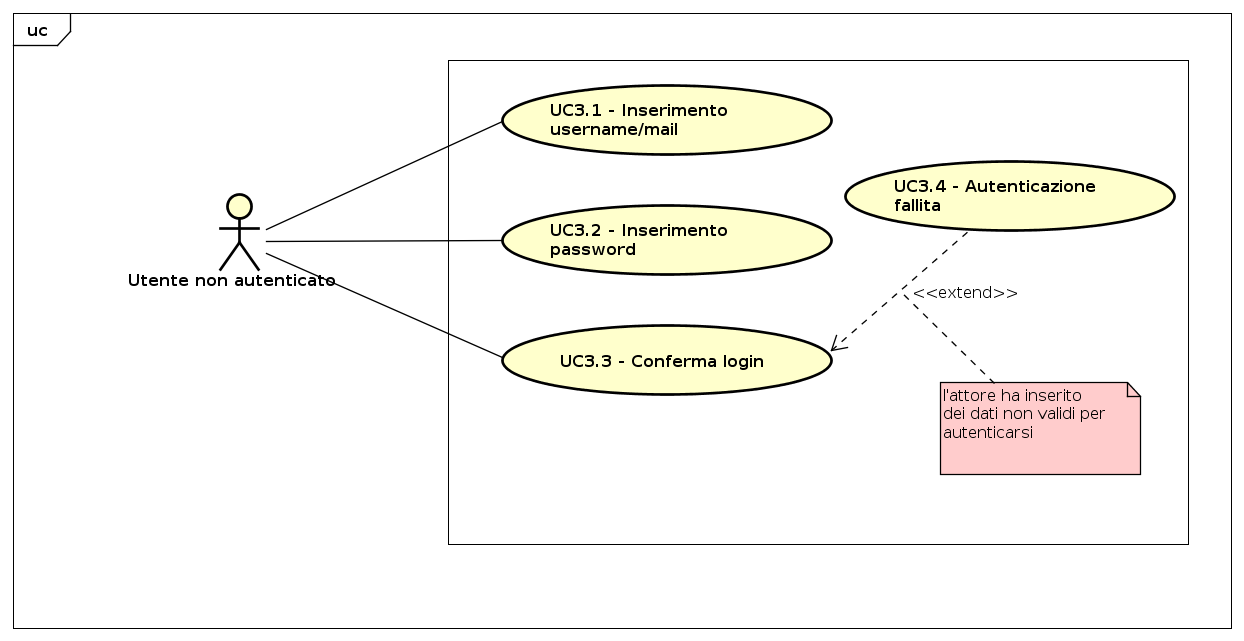
\includegraphics[scale=0.48]{UML/UC3.png}
	\caption{UC3: Login da \progetto}
\end{figure}
\FloatBarrier
\begin{itemize}
	\item \textbf{Attori}: utente non autenticato;
	\item \textbf{Descrizione}: l'attore si può autenticare inserendo username/mail e password, con cui è registrato;
	\item \textbf{Precondizione}: il sistema è avviato e pronto per l'utilizzo e mostra la pagina di login;
	\item \textbf{Postcondizione}: il sistema ha autenticato l'attore e quindi mostra all'attore autenticato la sua area riservata;
	\item \textbf{Scenario Principale}:
	\begin{enumerate}
		\item L'attore può inserire l'username oppure la mail utilizzata al momento della registrazione (UC3.1.1);
		\item L'attore può inserire la password (UC3.1.2);
		\item L'attore può confermare il login (UC3.1.3).
	\end{enumerate}
	\item \textbf{Estensioni}: autenticazione fallita (UC3.1.4).
\end{itemize}

\subsubsection{Caso d'uso UC3.1: Inserimento username/mail}
\begin{itemize}
	\item \textbf{Attori}: utente non autenticato;
	\item \textbf{Descrizione}: l'attore può inserire l'username o la mail associata al proprio account;
	\item \textbf{Precondizione}: il sistema presenta all'attore lo spazio destinato a questa operazione;
	\item \textbf{Postcondizione}: l'attore ha inserito username/mail;
	\item \textbf{Scenario principale}: l'attore inserisce l'username o la mail associata al proprio account. 
\end{itemize}

\subsubsection{Caso d'uso UC3.2: Inserimento password}
\begin{itemize}
	\item \textbf{Attori}: utente non autenticato;
	\item \textbf{Descrizione}: l'attore può inserire la password associata al proprio account;
	\item \textbf{Precondizione}: il sistema presenta all'attore lo spazio destinato a questa operazione;
	\item \textbf{Postcondizione}: l'attore inserisce la password;
	\item \textbf{Scenario principale}: l'attore inserisce la password associata al proprio account.
\end{itemize}

\subsubsection{Caso d'uso UC3.3: Conferma login}
\begin{itemize}
	\item \textbf{Attori}: utente non autenticato;
	\item \textbf{Descrizione}: l'attore può confermare i dati inseriti per effettuare il login;
	\item \textbf{Precondizione}: l'attore ha inserito l'username/mail e la password;
	\item \textbf{Postcondizione}: l'attore è autenticato;
	\item \textbf{Scenario principale}: l'attore conferma i dati inseriti per effettuare il login con il proprio account.
\end{itemize}

\subsubsection{Caso d'uso UC3.4: Autenticazione fallita}
\begin{itemize}
	\item \textbf{Attori}: utente non autenticato;
	\item \textbf{Descrizione}: l'attore può visualizzare un messaggio d'errore nel caso si fossero verificati uno o più scenari alternativi durante la fase di autenticazione;
	\item \textbf{Precondizione}: il sistema ha ricevuto dei dati errati per l'autenticazione;
	\item \textbf{Postcondizione}: il sistema avvisa l'attore dell'errore verificatosi tramite un opportuno messaggio;
	\item \textbf{Scenario principale}: l'attore visualizza un messaggio d'errore.
\end{itemize}